\documentclass[12pt, a4paper]{article}
\usepackage[francais]{babel}
\usepackage{caption}
\usepackage{graphicx}
\usepackage[T1]{fontenc}
\usepackage{listings}
\usepackage{geometry}
\usepackage[colorlinks=true,linkcolor=black,anchorcolor=black,citecolor=black,filecolor=black,menucolor=black,runcolor=black,urlcolor=black]{hyperref}

% \usepackage{mathpazo} --> Police à utiliser lors de rapports plus sérieux

\usepackage{fancyhdr}
\pagestyle{fancy}
\lhead{}
\rhead{}
\chead{}
\rfoot{\thepage}
\lfoot{Martin Baumgaertner - Mikhaïl Karapetyan}
\cfoot{}

\renewcommand{\headrulewidth}{0.4pt}
\renewcommand{\footrulewidth}{0.4pt}

\begin{document}
\begin{titlepage}
	\newcommand{\HRule}{\rule{\linewidth}{0.5mm}} 
	\center 
	\textsc{\LARGE iut de colmar}\\[6.5cm] 
	\textsc{\Large R4ROM19}\\[0.5cm] 
	\textsc{\large Année 2022-23}\\[0.5cm]
	\HRule\\[0.75cm]
	{\huge\bfseries TP 3 - Ansible}\\[0.4cm]
	\HRule\\[1.5cm]
	\textsc{\large martin baumgaertner - mikhaïl karapetyan}\\[6.5cm] 

	\vfill\vfill\vfill
	{\large\today} 
	\vfill
\end{titlepage}
\newpage
\tableofcontents
\newpage
\section{Premier pas avec Ansible}
\subsection{Exercice 1}
\subsubsection{Question 1-2-3}
Le fichier d'inventaire a bien été crée comme demandé dans l'énoncé, ainsi 
que le playbook. Nous avons ensuite donc ensuite executé le playbook avec
cette commande \texttt{ansible-playbook -i inventory deploy\_nginx.yml}
Voici une capture d'écran pour que le serveur a bien été déployé.
\begin{figure}[h]
    \centering
    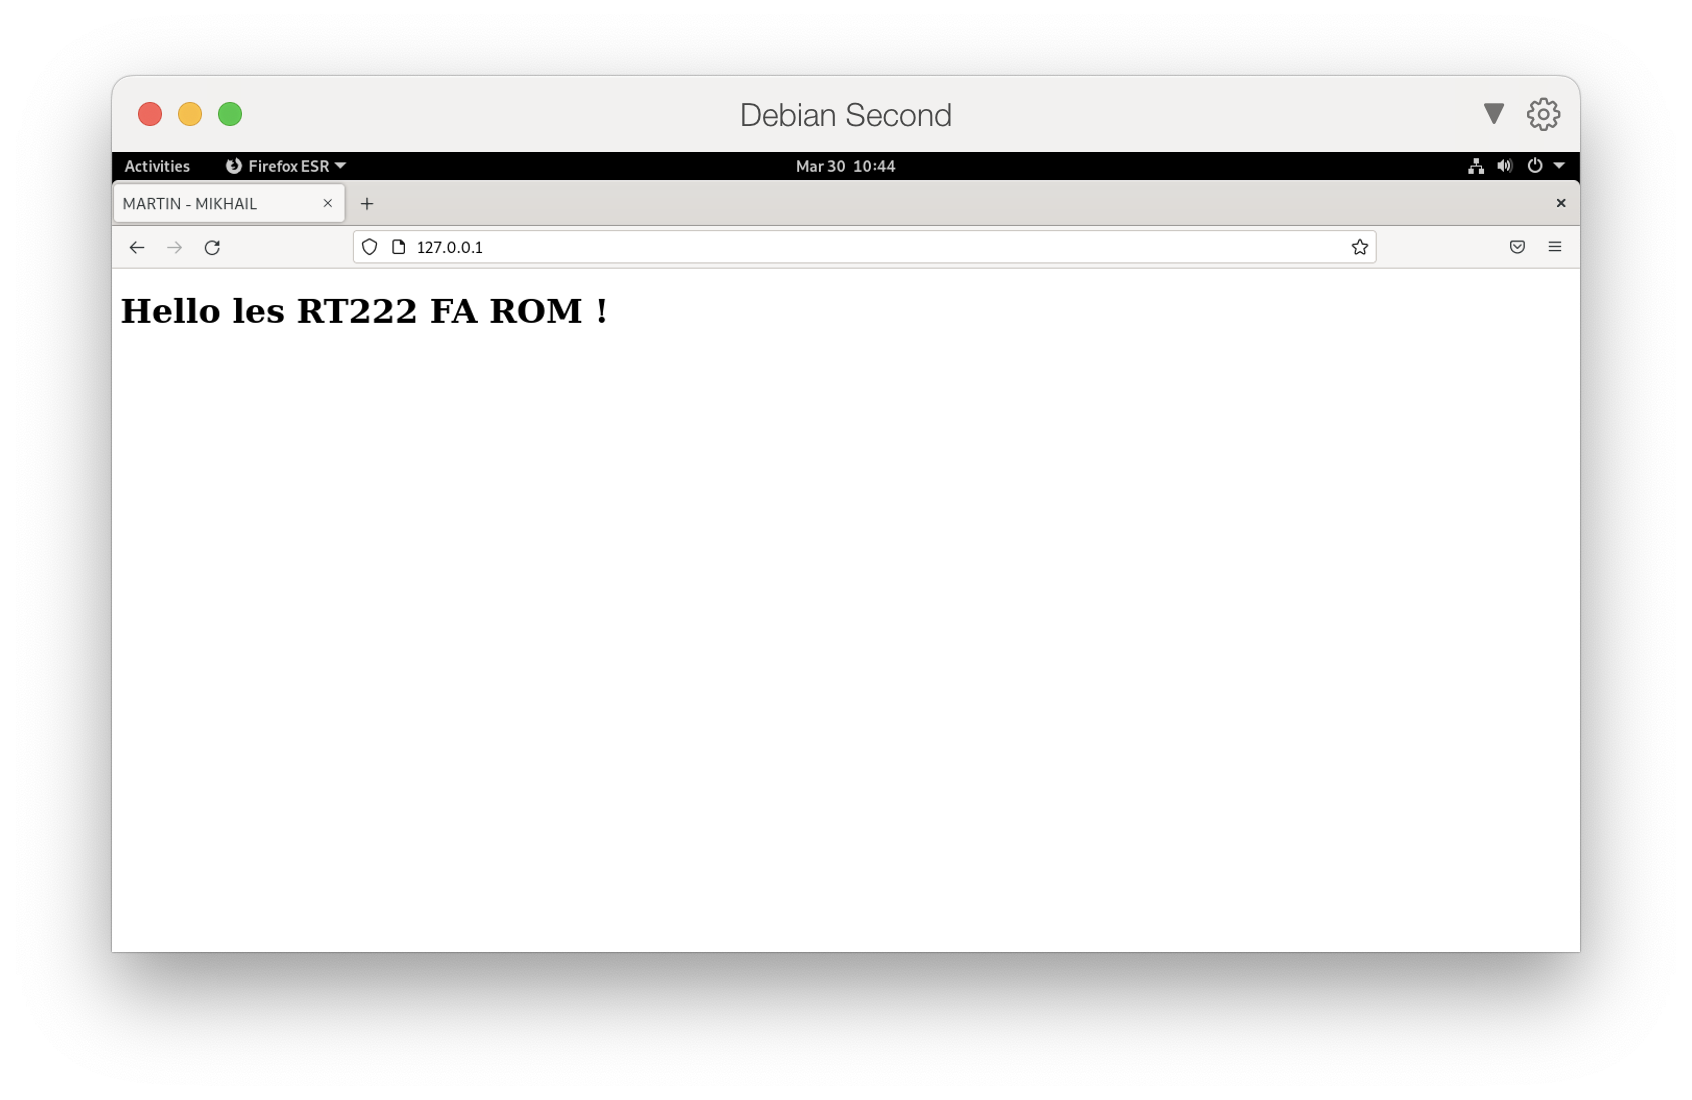
\includegraphics[width=1\textwidth]{img/nginx.png}
    \caption{Page HTML de nginx}
    \label{fig:1}
\end{figure}\\

Bien entendu, pour créer cette page il a fallu installer nginx sur le serveur 
et créer un script qui permet de faire fonctionner tous ces services. Voici
donc à la page suivante tous les éléments utilisés pour le fonctionnement 
de notre serveur Nginx. 

\newpage
Voici ensuite le script de déploiement de nginx, ainsi que le fichier d'inventaire
avec les informations du serveur distant. \\

\texttt{[servers]
serverngix ansible\_host=10.211.55.4 ansibl\_user=parallels ansible\_password=test1234}
\begin{figure}[h]
    \centering
    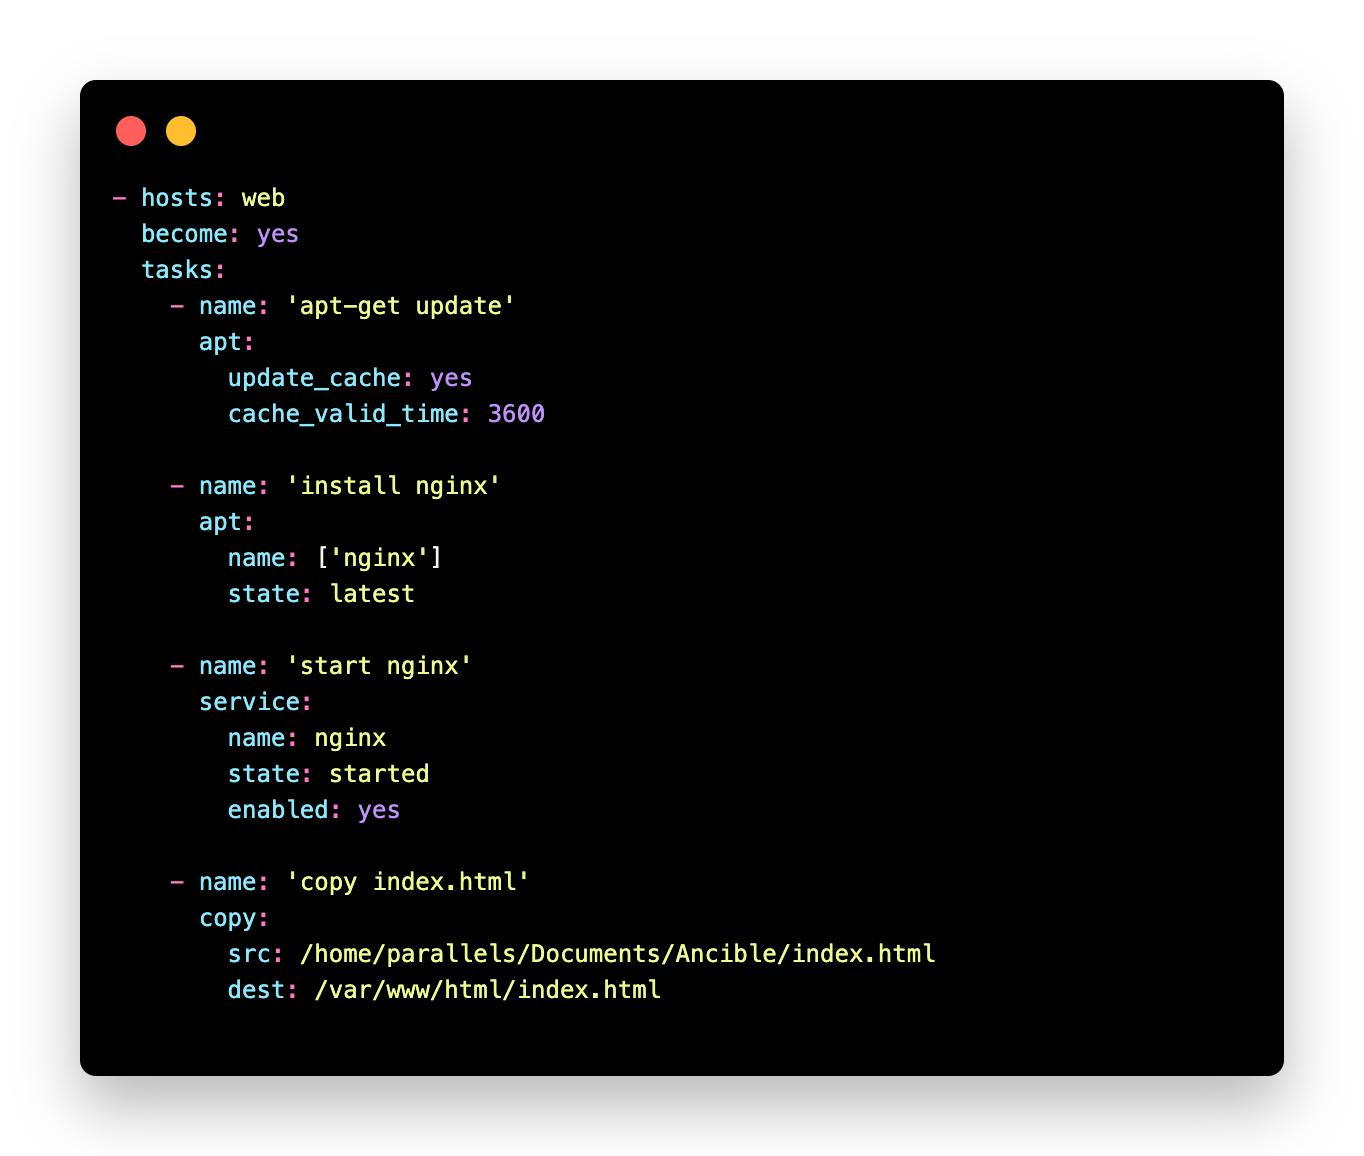
\includegraphics[width=1\textwidth]{img/deplou.png}
    \caption{Script de déploiement de nginx}
    \label{fig:1}
\end{figure}

\newpage
\section{Exercice 2}
Premièrement j'ai crée l'inventaire comme demandé avec 2 groupes, un pour les 
serveurs web et un pour les bases de données, en précisant que chaque 
groupe doit avoir au moins une machine. Voici le fichier d'inventaire :\\

[webservers]
web ansible\_host=10.211.55.4 

ansible\_user=parallels ansible\_password=test1234\\

[dbservers]
db ansible\_host=10.211.55.4 

ansible\_user=parallels ansible\_password=test1234\\

Ensuite, j'ai crée un rôle pour l'installation et la configuration de Apache.
Voici le fichier \texttt{main.yml} du rôle :\\
\begin{figure}[h]
    \centering
    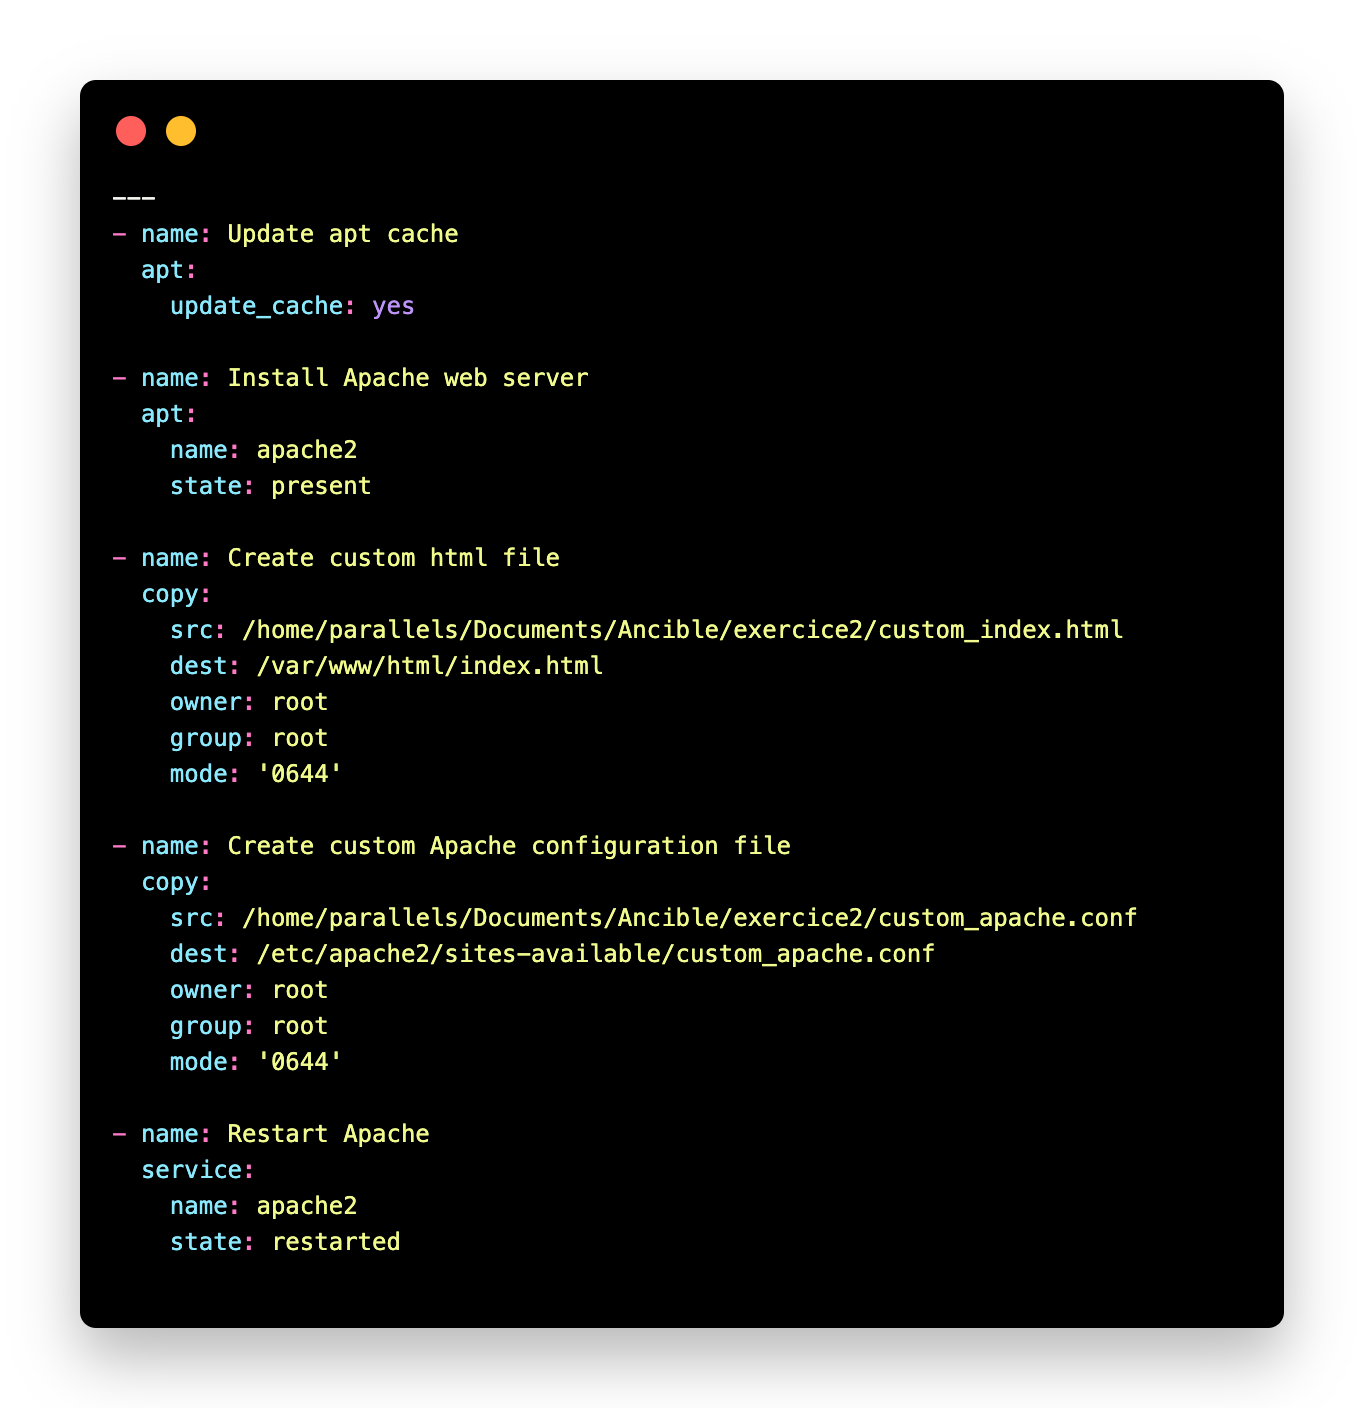
\includegraphics[width=0.6\textwidth]{img/yaml-apache.png}
    \caption{main.yaml}
    \label{fig:1}
\end{figure}

\newpage
Le fichier de configuration de Apache, et le fichier de configuration de MySQL. 
Ceci vont servir à créer 
\begin{figure}[h]
	\centering
	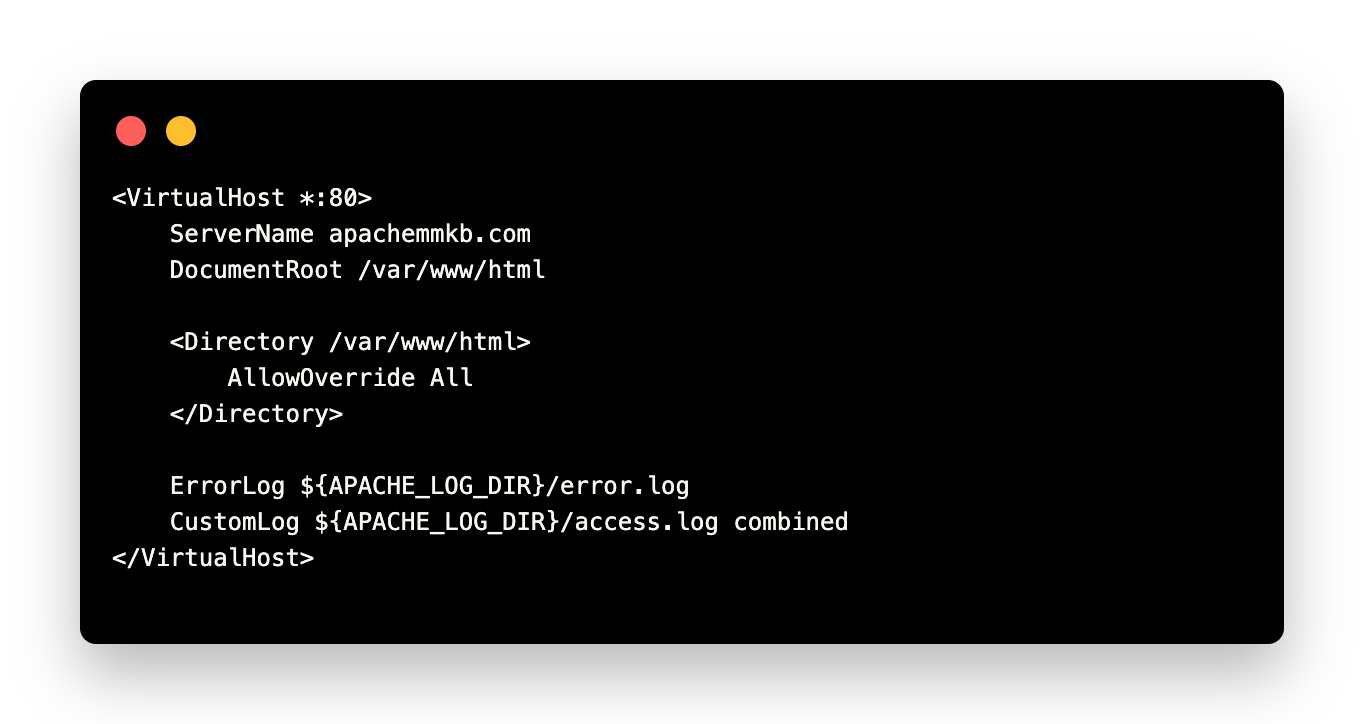
\includegraphics[width=1\textwidth]{img/apache-conf.png}
	\caption{apache.conf}
	\label{fig:1}
\end{figure}
\begin{figure}[h]
	\centering
	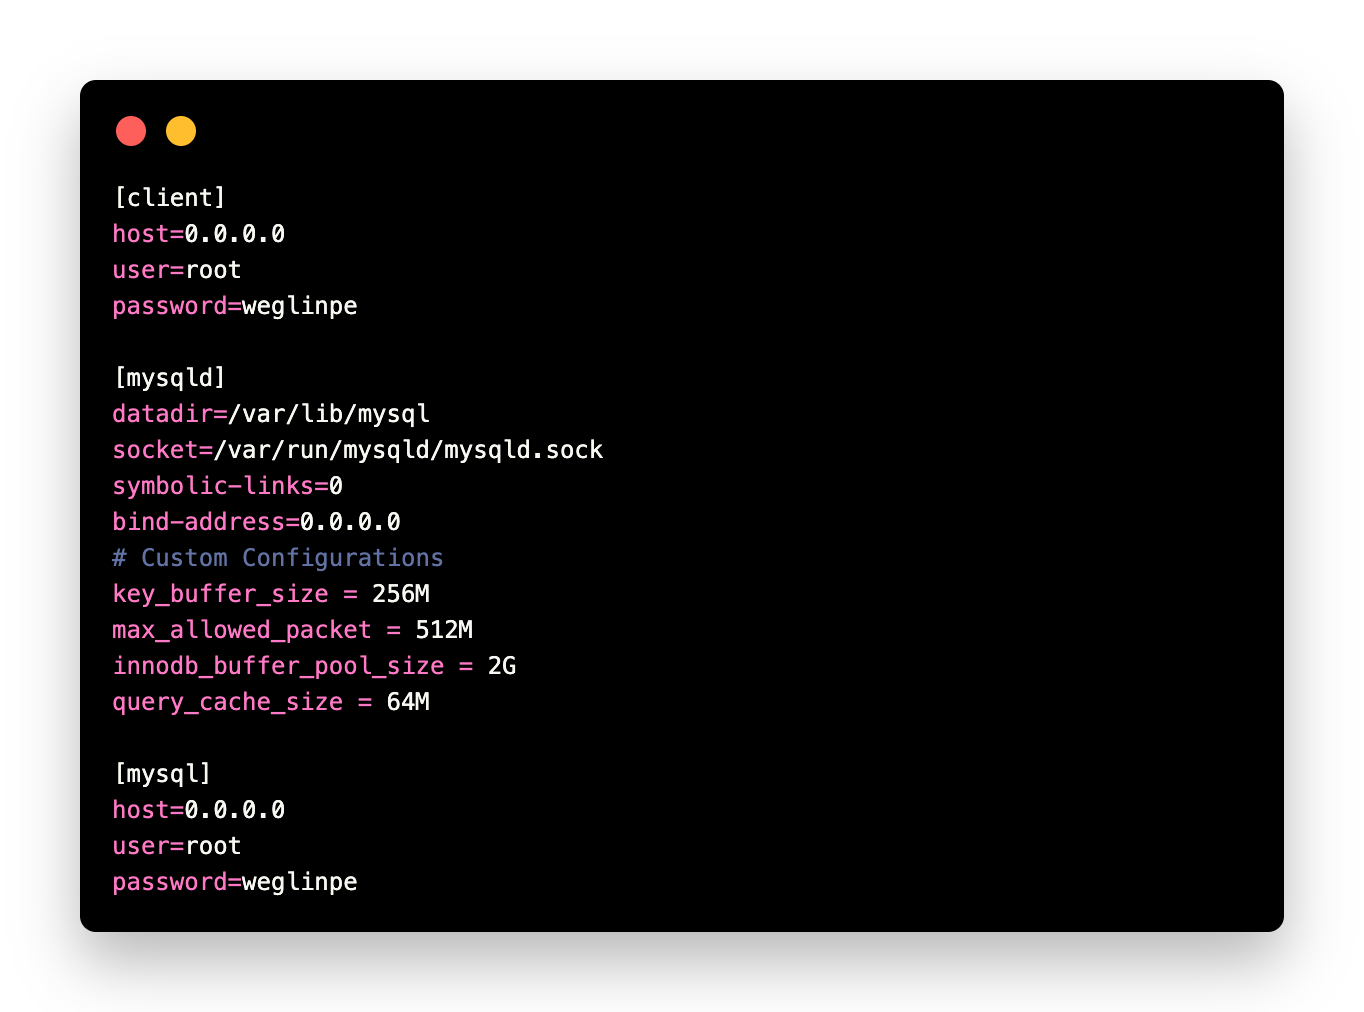
\includegraphics[width=0.5\textwidth]{img/my.png}
	\caption{my.conf}
	\label{fig:1}
\end{figure}

\newpage
Voici ensuite la configuration du rôle pour MySQL avec la fichier 
\texttt{main.yaml}\\
\begin{figure}[h]
	\centering
	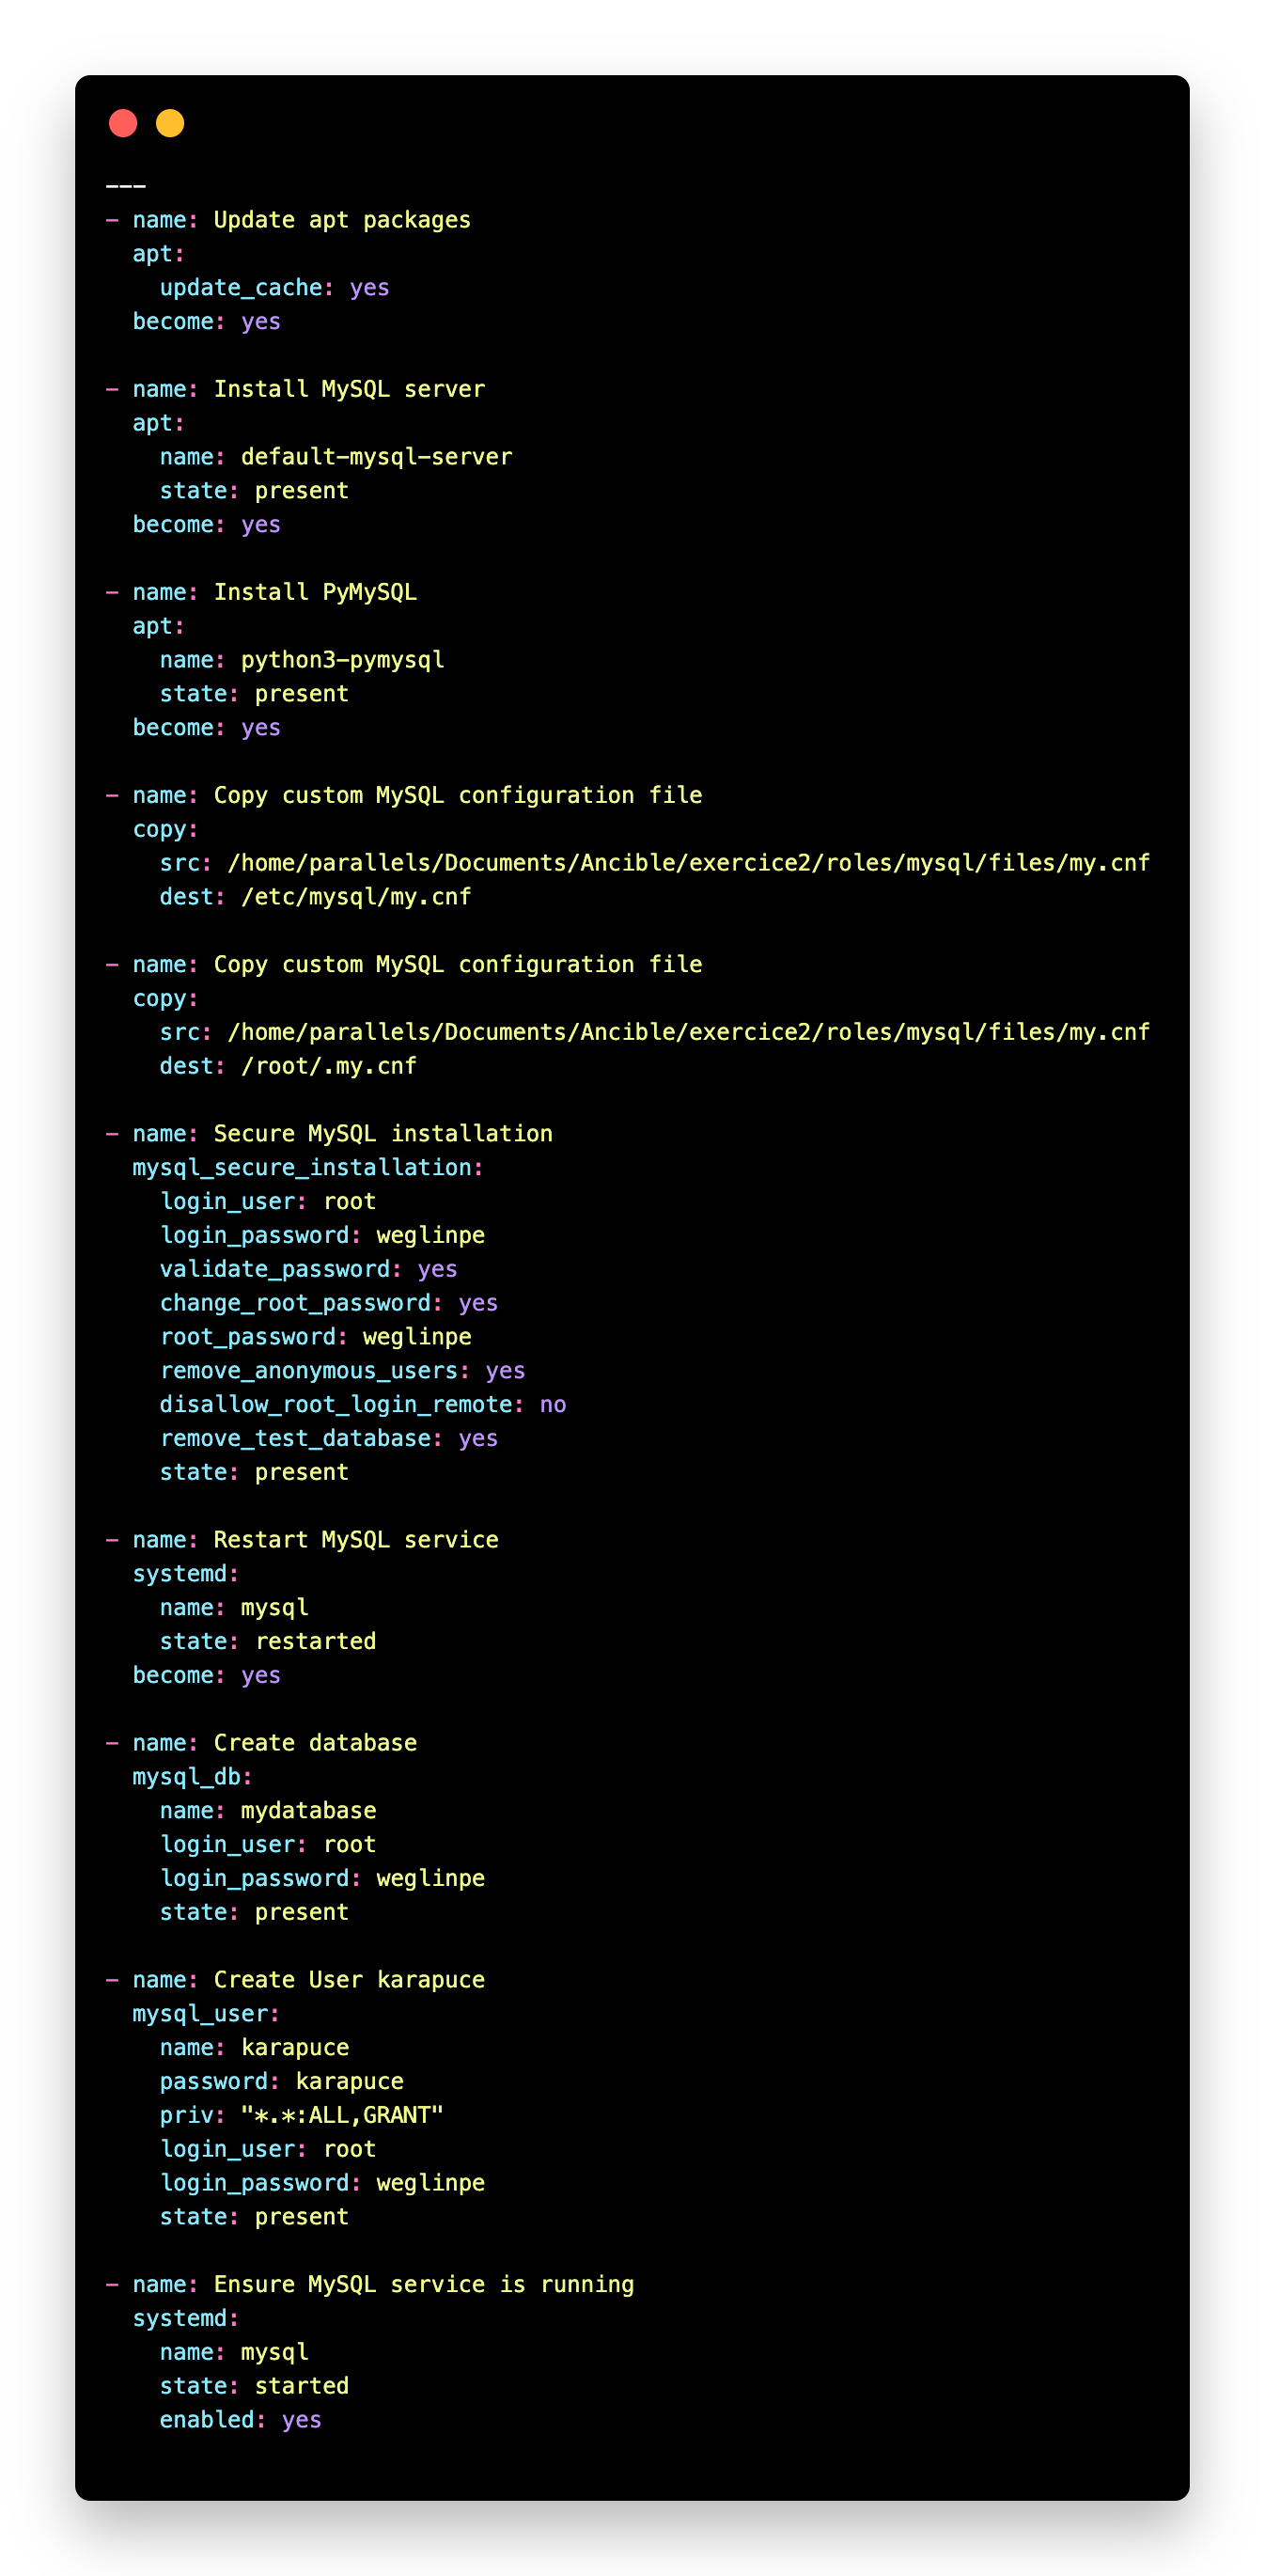
\includegraphics[width=0.5\textwidth]{img/mysql.png}
	\caption{main.yaml}
	\label{fig:1}
\end{figure}

Tous les fichiers de configurations, que ce soit ceux de apache ou de de mysql se trouvent dans 
\texttt{/roles/mysql/files} ou dans \texttt{/roles/apache/files}

\newpage
\section{Exercice 3}
\subsection{Question 1}
Voici donc le fichier dockerfile crée : 
\begin{figure}[h]
	\centering
	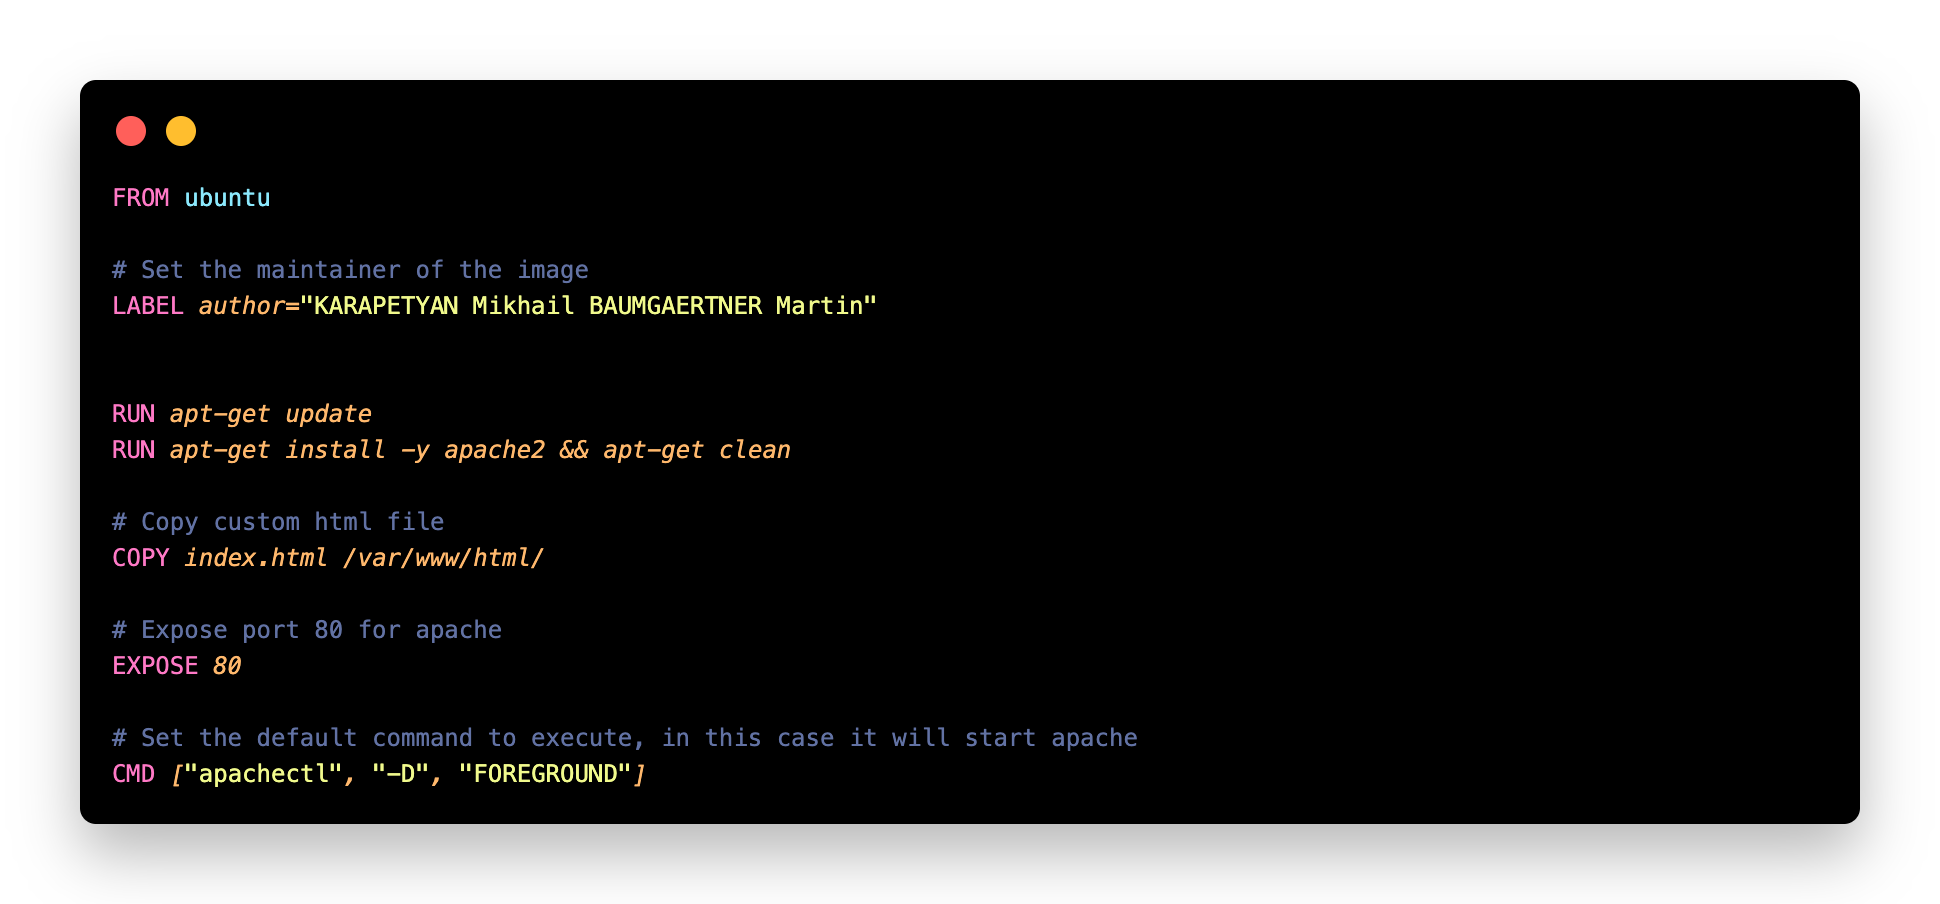
\includegraphics[width=1\textwidth]{img/dockerfile.png}
	\caption{dockerfile}
	\label{fig:1}
\end{figure}\\
Et voici le fichier html personnalisé :
\begin{figure}[h]
	\centering
	
\includegraphics[width=1\textwidth]{img/html.png}
	\caption{html}
	\label{fig:2}
\end{figure}

\newpage
\subsection{Question 2}
Pour créer le playbook ansible, il faut d'abord créer le fichier inventory.txt que voici : \\

\texttt{[servers]
serverapache2 ansible\_host=10.211.55.4 ansible\_user=parallels ansible\_password=1234toto}

Et voici ensuite le playbook ansible :
\begin{figure}[h]
	\centering
	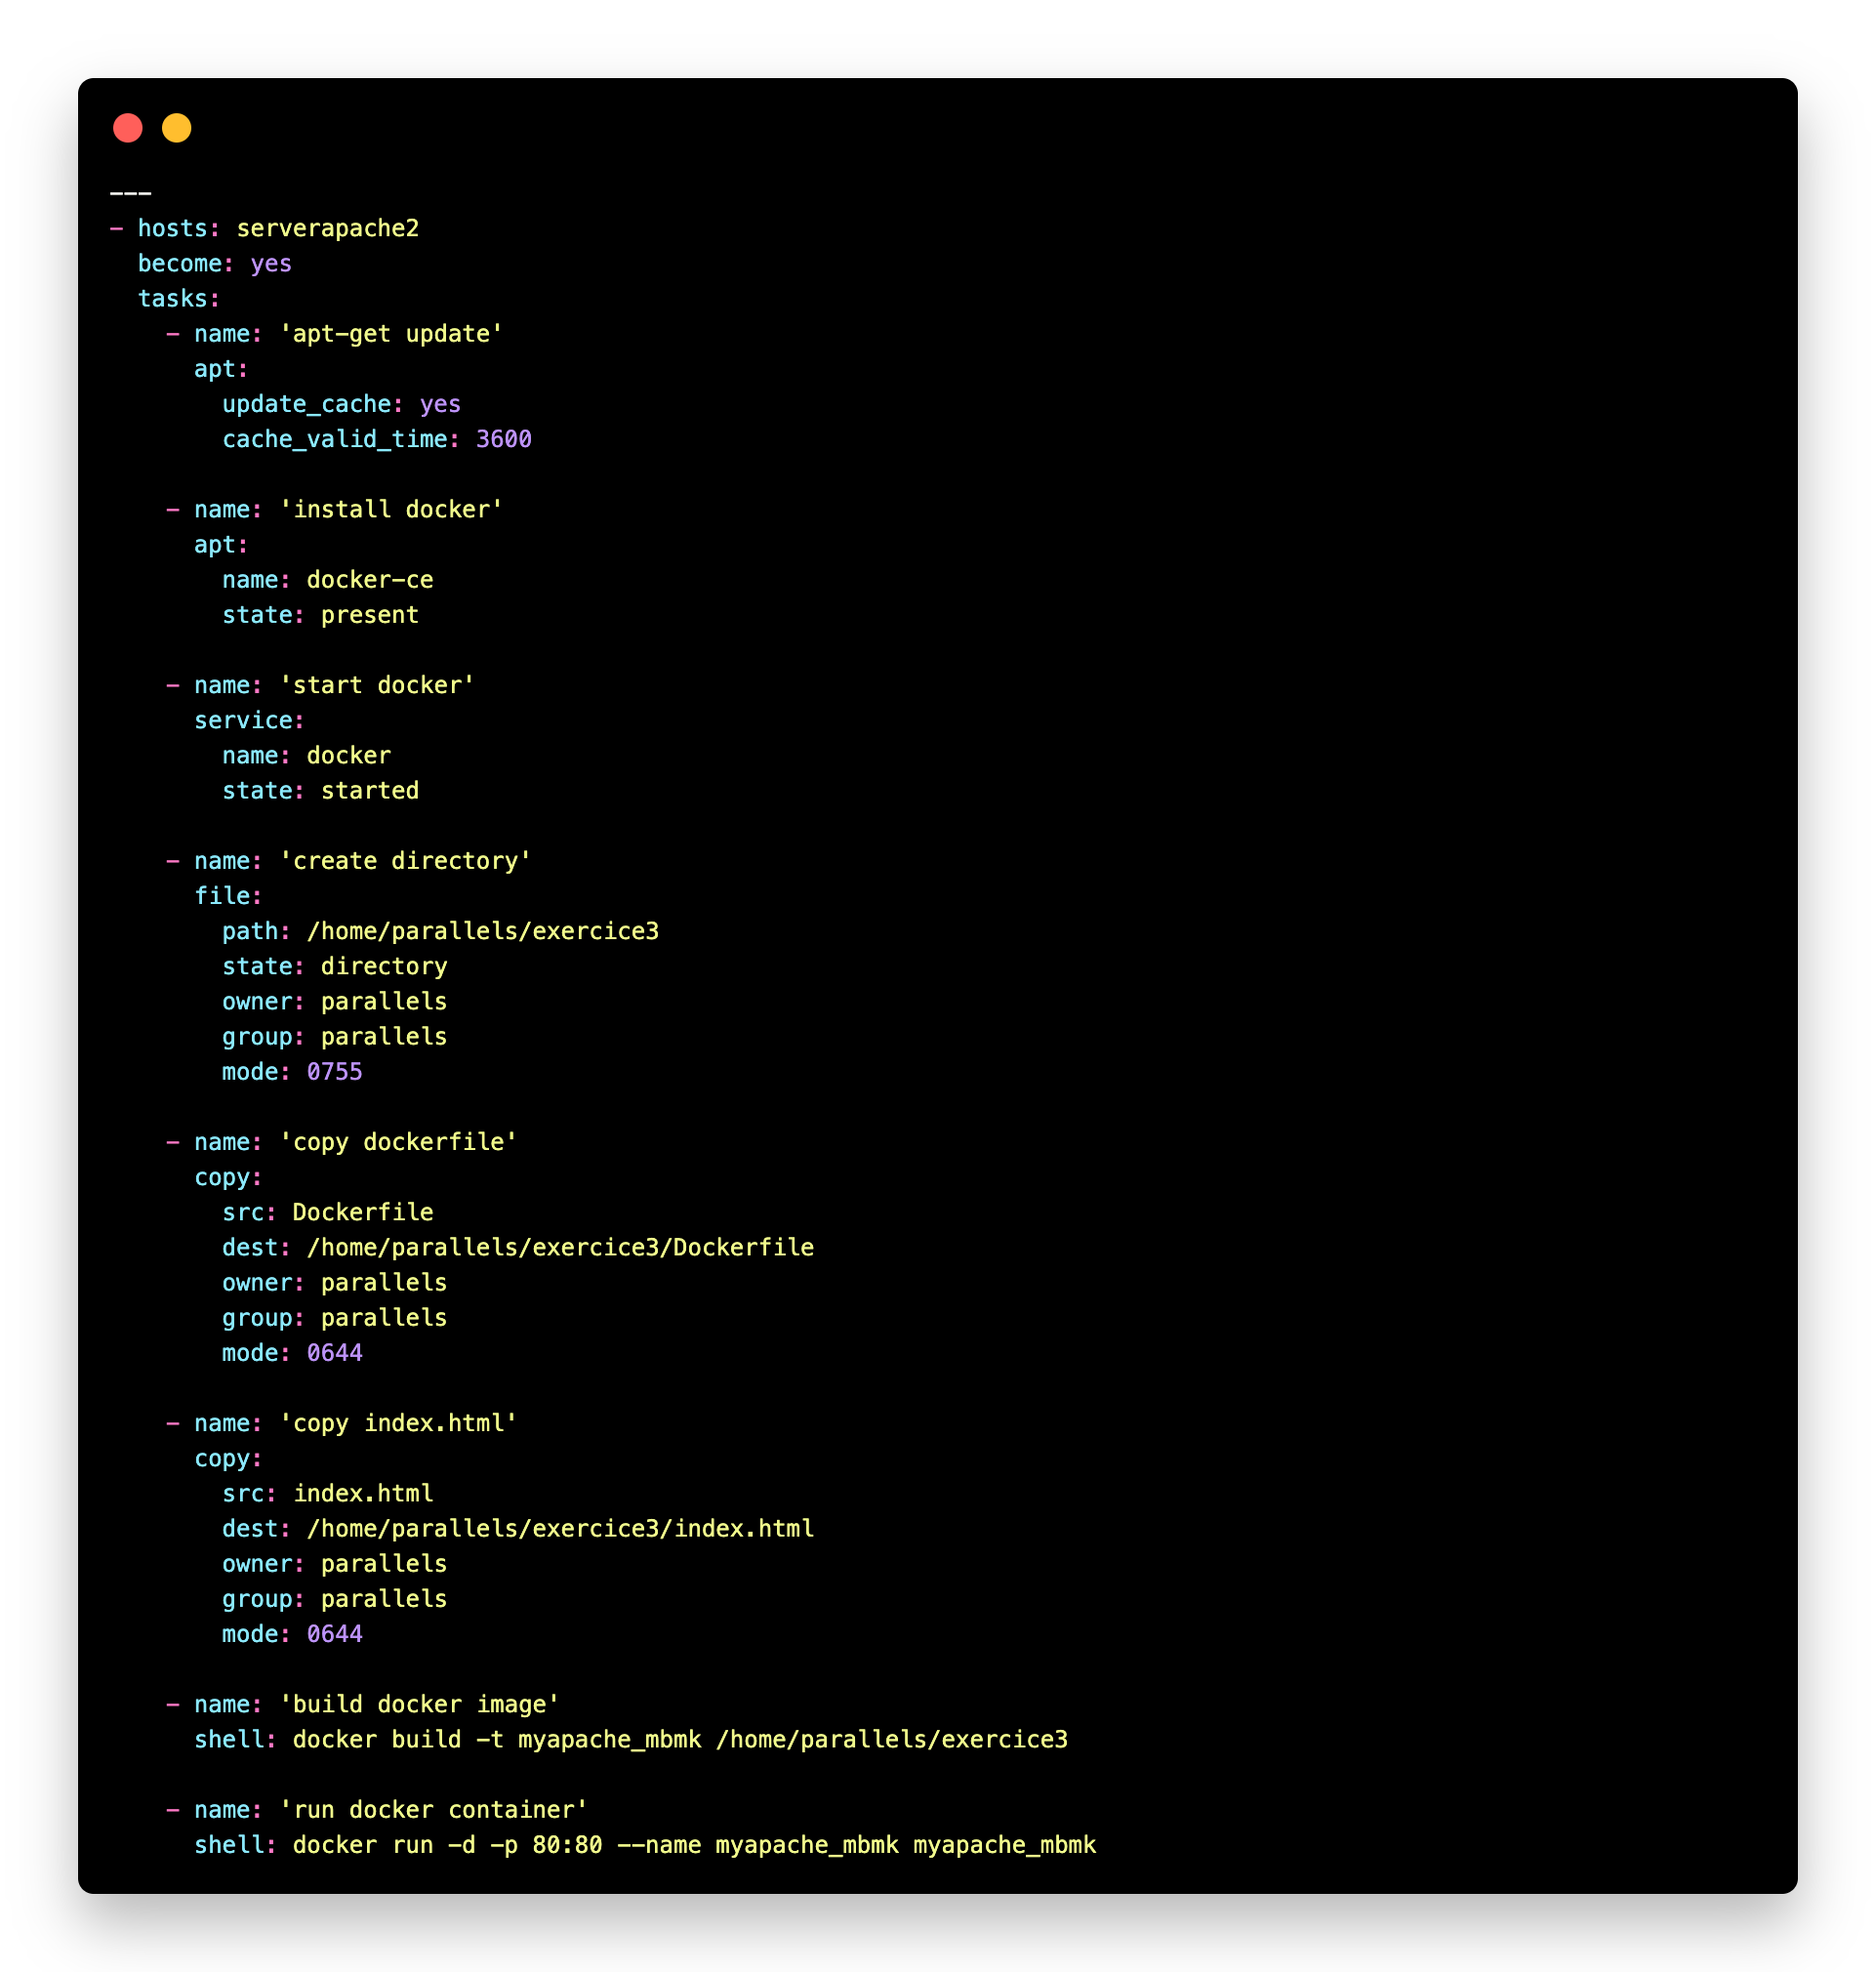
\includegraphics[width=0.9\textwidth]{img/playbook.png}
	\caption{deploy\_apache\_by\_docker.yml}
	\label{fig:3}
\end{figure}

\newpage
\subsection{Question 3-4}
Pour executer le playbook ansible, il faut au préalable placer tous ses fichiers sont 
dans un seul et meme dossier. Le playbook ansible est executé avec la commande suivante :\\

\texttt{ansible-playbook -i inventory.txt deploy\_apache\_by\_docker.yml}\\

Une fois le playbook executé, on peut voir que le container est bien lancé et qu'il est accessible depuis le navigateur web.

\subsection{Question 5}
Voici les modifications apportées pour correspondre à la demande de l'énoncé :\\
\begin{figure}[h]
	\centering
	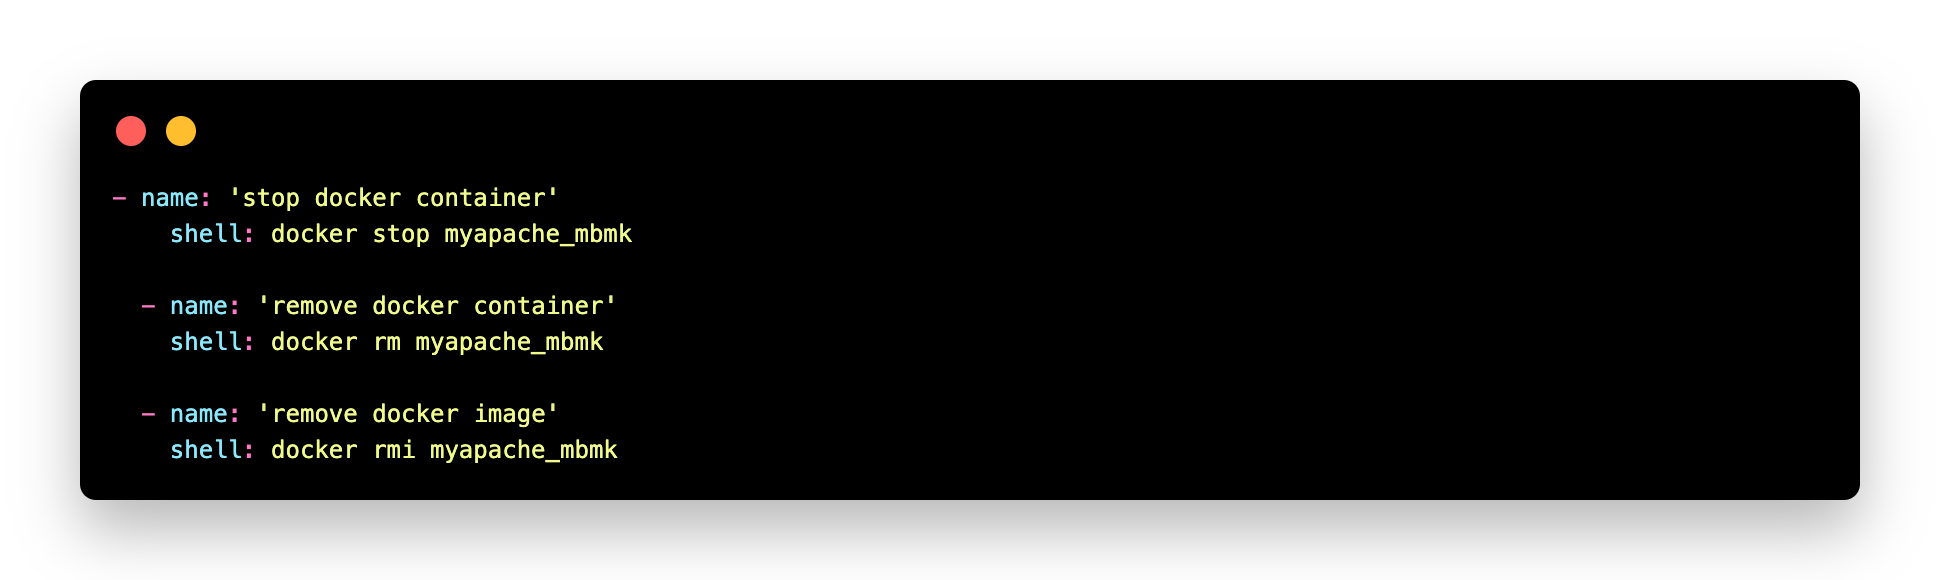
\includegraphics[width=1\textwidth]{img/modif.png}
	\caption{modifications}
	\label{fig:4}
\end{figure}



\end{document}